\documentclass[article,oneside]{memoir}

\usepackage{amsmath}
\usepackage{amssymb}
\usepackage{cclicenses}
\usepackage{color}
\usepackage{euler}
\usepackage[colorlinks=true,linkcolor=blue,citecolor=red]{hyperref}
\usepackage{float}
\usepackage{framed}
\usepackage[letterpaper,margin=2.5cm]{geometry}
\usepackage{graphicx}
\usepackage{inconsolata}
\usepackage{indentfirst}
\usepackage{libertine}
\usepackage[final]{microtype}
\usepackage{multicol}
\usepackage{nameref}
\usepackage{tabularx}
\usepackage{textcomp}
\usepackage{todonotes}


% PAGE SETUP
\setlength{\parindent}{5mm}
\nonzeroparskip
\raggedbottom
\raggedcolumns

% CONFIG FOR TOC, BIBLIO, ETC
\setcounter{tocdepth}{2}
\renewcommand{\bibname}{References}

% HANDY DEFINITIONS
\newcommand{\note}[1]{ \begin{framed} #1 \end{framed} }
\newcommand{\refdes}[1]{\texttt{#1}}
\newcommand{\mr}[1]{\ensuremath{\mathrm{#1}}}

\title{Owner's Manual}
\author{WCP52}

\begin{document}

\pagestyle{headings}
\begin{titlingpage}
%\setlength\extrarowheight{10mm}
\begin{tabularx}{\textwidth}{Xr}
\hline
\\
{\LARGE OWNER'S AND SERVICE MANUAL} &
Gain/Phase Analyzer \\
\\
\hline
\end{tabularx}
\vfill
\begin{center}
\missingfigure[figwidth=4in]{Photo}
\end{center}
\vfill
\begin{center}
\textcopyright 2015, Christopher Pavlina. Licensed under a Creative Commons Attribution 4.0 International License.
\end{center}
\end{titlingpage}

\begin{multicols}{2}

\tableofcontents
\listoffigures

\newpage
\input{intro/intro}

\newpage
\input{specifications/specifications}

\newpage
\input{oper/oper}

\newpage
\end{multicols}
\newpage
\begin{figure}[h]
\centering
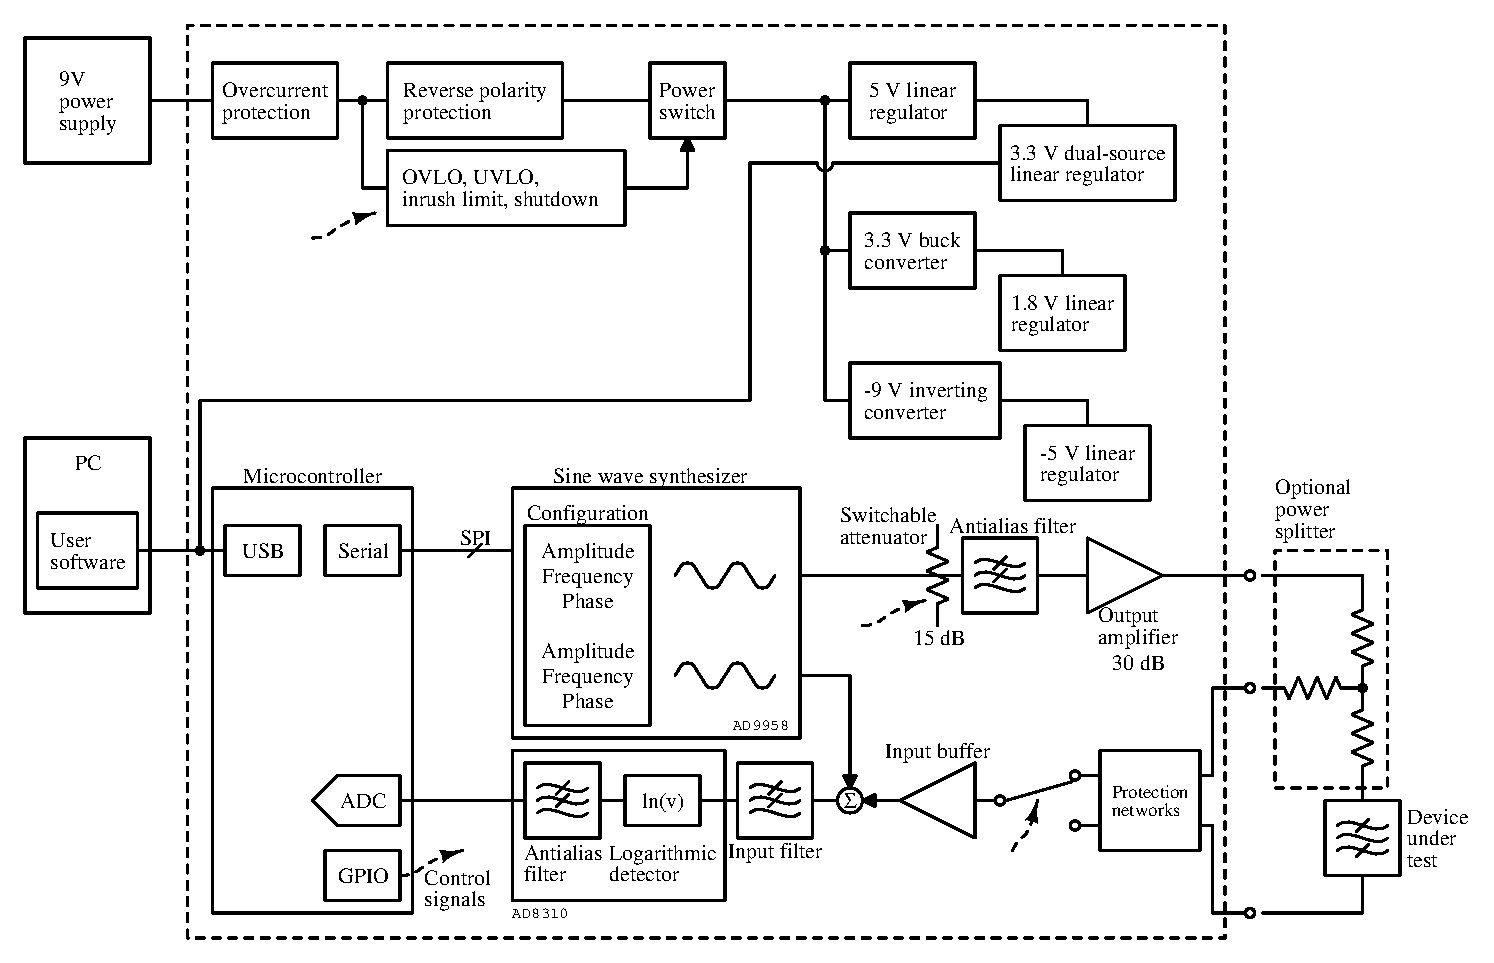
\includegraphics[width=6.5in]{blockdiagram}
\caption{Block diagram}
\label{fig:blockdiagram}
\end{figure}
\begin{multicols}{2}

\chapter{Theory of Operation}

This section contains a decription of the operation of the gain/phase analyzer.
Explanations range from simple and broad to very specific.
It is expected that the reader has an understanding of the basics of
gain/phase analysis itself, which is explained in the \hyperref[chap:intro]{Introduction
chapter}.

Also, it will be beneficial to look at the main system schematics when reading
through this section. Small pieces of the schematic are excerpted when helpful
in explaining their function, but are not always shown.

\section{Block Description}

The block diagram is shown in figure~\ref{fig:blockdiagram}. 


\section{Detailed Circuit Description}

\input{too/power}
\subsection{Synthesizer}

\schematicpage{3}{Synth}

In order to generate the test signals, a pair of sinusoids at anywhere from
1~kHz to above 150~MHz, the instrument uses a sophisticated
high-speed Direct Digital Synthesis (DDS) integrated circuit.

\begin{figure}[H]
\centering
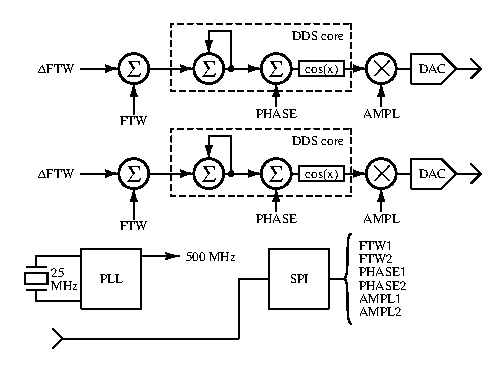
\includegraphics{dds}
\caption{DDS architecture}
\label{fig:dds}
\end{figure}

Figure~\ref{fig:dds} shows the internal architecture of the chip, somewhat
simplified from the version in the datasheet~\cite{ad9958}. In each of the two
independent waveform generators, a `frequency tuning word' (a 32-bit unsigned
integer) is repeatedly added to an accumulator at a rate of 500~MHz.
This causes the accumulator to increment, and overflow, at a higher rate for
higher tuning words. This sum is added to a phase offset, which allows each
signal to be independently offset from the other. This constantly incrementing
and resetting count is applied to a lookup table loaded with cosine values,
converting it from a digital ramp to a digital sinusoid. It is next multiplied
by an amplitude control value, and loaded into a digital-to-analog converter
(DAC) to generate the analog, sinusoidal waveform.

This integrated circuit is intended for radio applications. As such, it has
advanced features that this instrument does not require. It can be supplied
externally with a stable 500~MHz clock signal from a high quality
clock generator, but because we do not require such extreme stability, we
are instead using its internal Phase-Locked Loop (PLL) to multiply the clock
signal from a 25~MHz quartz crystal, \refdes{X1}, up to the full
internal clock frequency. Also, the device can generate modulated waveforms
using a 4-bit digital modulation input; these inputs are not used.

\subsection{Synthesizer Output Amplifiers}
\schematicpage{3}{Synth}

As is often the case with high-speed integrated circuits, the DDS chip has a
peculiar output system.

\begin{figure}[H]
\centering
\includegraphics{dds-output}
\caption{DDS output circuit}
\label{fig:ddsoutput}
\end{figure}

The outputs are symmetric current sinks, which pull up to 9.9~mA
down from AVDD (1.8~V), and the voltage that appears at these
outputs must not deviate by more than 500~mV from AVDD (or else
the signal will distort severely). The intended application is for these
to be connected to a center-tapped transformer, with the center tap connected
to AVDD. This is impractical due to the frequency range required: any
transformer with a high enough inductance to operate at 1~kHz has
too much parasitic capacitance to operate at 150~MHz. Instead,
a DC-coupled differential amplifier was used, with carefully designed
termination networks to provide the correct voltage range.

\begin{figure}[H]
\centering
\includegraphics{dds-outamp}
\caption{Output amplifier for synthesizer}
\label{fig:synthoutput}
\end{figure}

The 49.9~\Ohm{} resistors terminate the transmission line at the
source. The amplifier's inputs are relatively low impedance, so 53.6~\Ohm{}
resistors were used as load termination to provide a more accurate impedance when
placed in parallel with the differential amplifier.

Note that the input impedances of the two sides of the differential amplifier
are not equal. On the side entering the noninverting (`positive') input, the
impedance to ground is the sum of the two input resistors, or 720~\Ohm{}.
However, on the other side, the end of the feedback chain is not grounded, it is
a 180\dg{} phase-shifted copy of the input signal. The equivalent input impedance
here is only 360~\Ohm{}, and a more proper termination resistor there
would be 57.6~\Ohm{}. However, these transmission lines are very short,
and the difference in impedance does not make a significant difference. Using
two different resistors here would have increased the design complexity and cost,
and was deemed unnecessary. 
    

\subsection{Output System}
\schematicpage{4}{OutputAmp}

\subsubsection{Attenuator and Filter}
\subsubsection{Gain Stages and Termination}

\subsection{Input System}
\schematicpage{6}{InputFrontend}

\subsubsection{Protection}
\schematicpage{7}{Protection}

\subsubsection{Switching}

\schematicpage{8}{Switching}

It would not be practical for the analyzer to contain two independent input
subsystems to measure both inputs, as these systems are complex and expensive,
and there would be significant variation between the two. Instead, one input
subsystem is switched between two inputs. This switching is accomplished with a
pair of high-bandwidth SPST RF analog switches.

\begin{figure}[H]
\centering
\includegraphics{gaassw}
\caption{GaAs switch circuit}
\label{fig:gaassw}
\end{figure}

Figure~\ref{fig:gaassw} shows the internal circuit of the
switch~\cite{maswss0162}.  It is a simple circuit built from four gallium
arsenide (GaAs) FETs \footnote{The type of FET used is a relatively uncommon
    variant called a \emph{MESFET}, or MEtal-Semiconductor Field Effect
Transistor. This is a variant on the well known JFET, using a Schottky junction
instead of a PN junction. While uncommon in general, it is used often in GaAs
circuits due to the relative ease of constructing GaAs MESFETs.}.  These are
depletion-mode devices, so they are switched \emph{on} by applying zero volts
to the gate, and turned \emph{off} by applying a negative voltage, around
\Neg 5~V.  Switching on transistors \refdes{Q1} and \refdes{Q3} allows the
signal to pass through from the input to the output. Switching on transistors
\refdes{Q2} and \refdes{Q4} disconnects the input from the output, but also
\emph{terminates} the input (applies a $50\;\Omega$ resistance between the
input and ground). This is important to make sure that a disconnected input
does not cause signal reflections.

\begin{figure}[H]
\centering
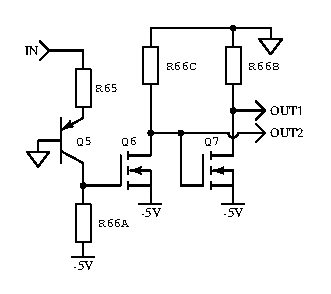
\includegraphics{gaasctl}
\caption{GaAs control circuit}
\label{fig:gaasctl}
\end{figure}

Figure~\ref{fig:gaasctl} is the control circuit for figure~\ref{fig:gaassw}.
When 0~V (a logic \emph{low}) is applied to the input from the
microcontroller, no current flows through \refdes{R65} or \refdes{R66A}.
This applies \Neg 5~V to \refdes{Q6}. Because \refdes{Q6}'s source is
connected to the \Neg 5~V rail instead of ground, the voltage between gate
and source ($V_{GS}$) is zero, and \refdes{Q6} is switched off.
This provides 0~V to one input of the GaAs switches. \refdes{Q7} acts
as an inverter, providing \Neg 5~V to the other GaAs switch input. The
dual switches have their inputs connected opposite each other, so this
switches one of them \emph{on} and the other \emph{off}.

When 3.3~V (a logic \emph{high}) is applied to the input from the
microcontroller, about 1.6~mA flows through \refdes{R65}. This
saturates \refdes{Q5}, applying about 0.7~V to \refdes{Q6}. As above,
$V_{GS}$ is the difference between this and the \Neg 5~V rail, or
5.7~V. \refdes{Q6} now switches on, and the two signals to the GaAs
switches swap places. This swaps the two switches, turning on the one that was
off, and turning off the one that was on.


\subsubsection{Buffer and Filter}
\schematicpage{9}{Buffer\_Filter}

\begin{figure}[H]
\centering
\missingfigure[figwidth=3in]{buffer}
\caption{Input buffer circuit}
\label{fig:buffer}
\end{figure}

Figure~\ref{fig:buffer} is the input signal buffer. \refdes{Q9} is a simple
emitter-follower (common collector) amplifier, providing isolation
between the input and further circuitry. \refdes{Q10} and \refdes{Q8} form
a current source to power it, in a feedback configuration providing
approximately $0.65\;\mr{V} / 30\;\Omega \approx 22\;\mr{mA}$.

The configuration of \refdes{R76} and \refdes{R77} sums together
the input signal and the phase reference signal, and this continues to the
input filter. \refdes{R75} combines with \refdes{R76} to properly
terminate the 50~\Ohm{} phase reference signal.

To lower the effect of external interference on the signals, a filter restricts
signals above the instrument's maximum operating frequency from continuing
past this point.

\subsubsection{Logarithmic Detector}
\schematicpage{10}{Detector}

\subsection{Microcontroller}
\schematicpage{13}{MPU}
\subsubsection{USB Communications}
\schematicpage{2}{Comm}




\section{Software Description}
\subsection{Signal Processing}
\subsubsection{Sampling}
\subsubsection{Null Search}
\subsubsection{Calibration}
\subsection{User Interface}




\end{multicols}

\newpage
\chapter{Full schematics}

\newpage
\begin{thebibliography}{9}

\bibitem{aod417}
Alpha \& Omega Semiconductor, ``AOD417 P-Channel Enhancement Mode Field Effect Transistor,''
AOD417 datasheet, 2008. \url{http://aosmd.com/pdfs/datasheet/AOD417.pdf}

\bibitem{tranckts-sawtooth}
S. W. Amos and M. James, ``Sawtooth generators,'' in
\emph{Principles of Transistor Circuits}, 9th ed. Oxford: Newnes, 2003, ch. 14, pp. 281--292.

\bibitem{ad9958}
Analog Devices, Inc., ``2-Channel, 500 MSPS DDS with 10-Bit DACs,'' AD9958 datasheet,
April 2013 [Revision B].
\url{http://www.analog.com/media/cn/technical-documentation/data-sheets/AD9958.pdf}

\bibitem{az1117c}
Diodes Incorporated, ``Low Dropout Linear Regulator,'' AZ1117C datasheet,
October 2014 [Revision 3--2].
\url{http://www.diodes.com/datasheets/AZ1117C.pdf}

\bibitem{aoe-vreg}
P. Horowitz and W. Hill, ``Voltage regulators and power circuits,'' in
\emph{The Art of Electronics}, 2nd ed. Cambridge: Cambridge, 1989, ch. 6, pp. 307--389.

\bibitem{maswss0162}
M/A-COM Technology, ``GaAs SPST Switch,'' MASWSS0162 datasheet [Revision V3].
\url{http://cdn.macom.com/DataSheets/MASWSS0162.pdf}

\bibitem{mcp1700}
Microchip Technology, ``Low Quiescent Current LDO,'' MCP1700 datasheet,
October 2013 [Revision C].
\url{http://ww1.microchip.com/downloads/en/DeviceDoc/20001826C.pdf}

\bibitem{mc79m00}
ON Semiconductor, ``500 mA Negative Voltage Regulators,'' MC79M00 series datasheet,
July 2013 [Revision 15].
\url{http://www.onsemi.com/pub_link/Collateral/MC79M00-D.PDF}.

\bibitem{l78m05}
STMicroelectronics, ``Precision 500 mA regulators,'' L78M datasheet, June 2014 [Revision 20].
\url{http://www.st.com/web/en/resource/technical/document/datasheet/CD00000447.pdf}

\bibitem{tl431}
Texas Instruments, ``TL43xx Precision Programmable Reference,''
TL431 datasheet, Aug. 2004 [Revised Jan. 2015]. \url{http://www.ti.com/lit/ds/symlink/tl431.pdf}

\bibitem{buckinv}
J. Tucker, ``Using a buck converter in an inverting buck-boost topology,''
\emph{Analog Applications Journal}, Texas Instruments, fourth quarter 2007, pp. 16--19.
\url{http://www.ti.com/lit/an/slyt286/slyt286.pdf}
\end{thebibliography}


\end{document}
